\section{Background}


% \subsection{Autonomous systems}
% 
% Autonomous systems are systems that are capable of changing their behaviour in
% response to unanticipated events during
% operation~\cite[368]{watson2005autonomous}. Autonomous systems exist in several
% different forms and they are typically tailored for their specific operating
% environments. Some systems operate in the maritime domain, some in the air, and
% others on the ground in the terrestrial operating domain~\cite[369-370]{watson2005autonomous}.

\subsection{\acrfull{ads}}

\acrfull{ads} are systems that enable automative vehicles to drive autonomously. Due to the
typical operating scenarios of a car it is pivotal that the \acrlong{ads} maintain a high safety standard. A common way to assert safety
is to use simulator based testing~\cite[1]{DeepScenario}.

\subsubsection{\acrlong{ad} testing}

Testing is essential for assuring \acrlong{ad} operative safety~\cite[163]{ADTestingReview16}.
Several methods for testing exist, testing various aspects of the \acrlong{ad}. An \acrshort{ad}
typically exists of several modules, all working together and handling different aspect of the
\acrlong{ad}.

\citeauthor{ADTestingReview16} outline several typical architectures for \acrshort{ad} testing,
drawing on traditional software testing traditions outlining how \textit{software testing} can be
used alongside more specialized \acrshort{ad} testing techniques such as \textit{simulation testing}
and \textit{X-in-the-loop testing}~\cite[163-164]{ADTestingReview16}.

\subsubsection*{\acrlong{ad} driveability}\label{sec:adsDrivability}

\textbf{Driveability} is a high-level estimator of the overall driving
condition of an \acrshort{ad}, derived from several lower-level sources~\cite[3140]{safeToDrive}.
It can be used to refer to various aspects of a scene.
\citeauthor{safeToDrive} discuss the concept further, using the  scene definition
of~\citeauthor{scenes} as outlined in  \cref{sec:adsSimConcepts}, they describe
how driveability can refer both to \begin{inparaenum}
    \item road conditions, and
    \item human driver performance.
\end{inparaenum}
\citeauthor{safeToDrive} go on to give an overview of how driveability
can be used to refer to a \begin{inparaenum}\setcounter{enumi}{2}
    \item \textit{driveability map} which divides a map into
    cells indicating where the \acrshort{ad} expects that it will be able to go, and
    \item \textit{object driveability}, which refers to the classification of physical
    objects in the environment that the \acrshort{ad} expects that it can run over
    without causing damage to the ego vehicle~\cite[3135-3136]{safeToDrive}.
\end{inparaenum}

The main method for the assessing driveability of a scene comes form assessing the environment
of the scene. Factors such as \begin{inparaenum}
    \item wheather,
    \item traffic flow,
    \item road condition,
    \item obstacles
\end{inparaenum} all play into this. The \acrshort{ad} infers information from
observation~\cite[3136]{safeToDrive}.

They continue to give an overview of various \textit{driveability factors} and
their associated difficulties, using a a split between \textit{explicit} and
\textit{implicit} factors.

\textbf{Explicit driveability factors} will typically include factors such as
\textbf{Extreme wheather} such as \begin{inparaenum}
    \item fog,
    \item heavy rain,
    \item snow,
\end{inparaenum}
all serving to impair road visibility and causuing increased difficulties for
vision-based tasks such as road detection and object
tracking~\cite[3136-3137]{safeToDrive}. \textbf{Illumination} also poses
various challenges for typical \acrshort{ad} tasks as a typical \acrshort{ad}
will be required to operate in a plethora of scenes with varying degrees of
illumination depending on factors such as time of day and location (e.g. if the
\acrshort{ad} is operation in a dimly lit tunnell)~\cite[3137]{safeToDrive}. The
authors highlight how low illumination may serve as an advantage for the
\acrshort{ad} as this allows for using the head lights of other vehicles as a
feature for detecting them, wheras it make pedestrian detection significantly
more challenging~\cite[3137]{safeToDrive}. \textbf{Road geometry} is another
external factor, satisfying our natural intuition that \textit{intersections}
and \textit{roundabouts} are more difficult to drive through than straight
highways~\cite[3137]{safeToDrive}.

\textbf{Implicit driveability factors} consist of behaviors and intent of other road users
interacting with the autonomous car~\cite[3138]{safeToDrive}. This includes the actions of other
vehicles such as their \begin{inparaenum}
    \item overtaking,
    \item lane changing,
    \item rear-ending,
    \item speeding, and
    \item failure to obey traffic laws \end{inparaenum}.~\citeauthor{safeToDrive} call these factors
\textbf{vehicle behaviours}~\cite[3138]{safeToDrive}. Furhtermore, \textbf{pedestrian behaviours}
are also taken into account, noting how pedestrians can sometimes
\begin{inparaenum}\setcounter{enumi}{5}
    \item cross the road,
    \item be inattentive, or
    \item fail to comply with the traffic law \end{inparaenum}\cite[3138]{safeToDrive}. They go on
to describe the \textbf{driver behaviour} of other drivers pointing out how
\begin{inparaenum}\setcounter{enumi}{8}
    \item distraction, and
    \item drowziness \end{inparaenum} can be factors that caus accidents even for
\acrshort{ad}-enhanced vehicles due to the other, manual, cars
interfering with their operation~\cite[3138-3139]{safeToDrive}. Lastly
\textbf{motorcyclist/bicyclist behaviours} cause their own source of implicit driveability factors:
The models and methods developed for analysing the group's behaviour are far more limited than other
groups of road users~\cite[3139]{safeToDrive}.~\citeauthor{safeToDrive} theorise that this comes
down to the lack of available dataset thats that capture and label the trajectories and behaviours
of motorcyclists and bicyclists~\cite[3139]{safeToDrive}, causing potential issues for any
\acrshort{ad} that wishes to operate in a shared traffic environment with this group.

\subsubsection*{\acrlong{ad} testing metrics}\label{sec:adsMetrics}

When evaluating \acrshort{ad} testing, several metrics can be used. What metric to use will depend
on what the relevant test is measuring.

Building on what we have learnt about driveability (\cref{sec:adsDrivability}),
we take after \citeauthor{safeToDrive} and review three metrics for
quantifying driveability: \begin{inparaenum}
    \item scene driveability,
    \item collision-based risk, and
    \item behaviour-based risk.
\end{inparaenum}

\textbf{Scene driveability} refers to how easy a scene is for an
\acrshort{ad} to navigate, and the \textit{scene driveability score} refers to
how likely the \acrlong{ad} is to fail at traversing thhe
scene~\cite[3140]{safeToDrive}. It is typically found through and end-to-end
approach. Note how this is a metric for \textit{scenes}, without taking into
account the performance of any specific \acrshort{ad}.

\textbf{Collision-based risk} comes in two kinds - \begin{inparaenum}
    \item binary risk indicator, and
    \item probabilistic risk indicator.
\end{inparaenum} \citeauthor{safeToDrive} posit that the prior, binary metric, indicates wheter a
collision will happen in the near future in a binary `either-or' sense, wheras the latter yields a
probability calculated based on current states, event, choice of hypothesis, future states and
damage~\cite[3140]{safeToDrive}.

\textbf{Behaviour-based risk} estimation also represents a binary classification problem wherein
nominal behaviours are learnt from data, and then dangerous behaviours are detected on that. This
requires a definition of `nominal behaviour', which is typically defined on on acceptable speeds,
traffic roles, location semantics, weather conditions and/or the level of fatique of the
driver~\cite[3140]{safeToDrive}. Furthermore \citeauthor{safeToDrive} describe how this metric also
allows more than one \acrshort{ads} to be labelled as `conflicting' or `not
conflicting'~\cite[3140]{safeToDrive}, representing a ruling on their compatibility. Finally, they
note how behaviour-based risk assessment typically focuses on driver behaviours, not taking into
account other actors in the scene such as pedestrians or cyclists.

%Furthermore, \citeauthor{safeToDrive} also give an overview of metrics and their relevant factors.
%Furthermore, \citeauthor{safeToDrive} also give an overview of metrics and their relevant factors.


% \tanke{This can be expanded if needed}

\subsubsection*{The complexities of \acrshort{ad} testing}\label{sec:adsTestingComplexity}

As we have seen, \acrshort{ads} can perform several tasks, in several environments. As such, there
are several relevant factors for testing them. It is not feasible to test all potential variations
of all potential environments in the real world, meaning that the \textit{test
    coverage}\footnote{See \cref{sec:testCoverage}} typically will be low.

Some of the factors that complicate \acrshort{ad} operations are \begin{inparaenum}
    \item timing,
    \item sequence of events, and
    \item parameter settings such as the different speeds of various vehicles and other actors.
\end{inparaenum}

\citeauthor{adsComplexityIndex18} posit that \textit{the concept of complexity exists everywhere,
    but there is no agreement on one for driving situations}~\cite[1182]{adsComplexityIndex18}.
Therefore they introduce their own concept of \acrfull{dsc}, which serves to give a metric of a
the complexity of a given driving situation. Their \acrshort{dsc} is defined as the output of a
mathematical formula taking into account the perplexity and standard deviation of several
control variables $\mathcal{M}$ representing the surrounding vehicles's
behaviour~\cite[1182]{adsComplexityIndex18}. Their formula also takes into account the ratio of
\textit{V2X}-capable vehicles~\cite[1182]{adsComplexityIndex18}, i.e. the vehicles that are
connected and capable of communicating~\cite[1]{v2xTestingSurvey2019}.

% It is common to modularize the testing of \acrshort{ads} so that the individual modules can be
% tested in isolation. The modules of an \acrshort{ad} typically include a motion planner, a
% \acrfull{cv} system, and % LIDAR. This allows for testing the individual modules in a way that
% makes sense for their specific domains.

\subsubsection{\acrlong{ad} simulation}

Due to the complexity involved in testing \acrlong{ads} (\cref{sec:adsTestingComplexity}),
simulators are typically used for this purpose~\cite{DeepScenario}. While the same points about not
being able to test \textit{all} possible scenarios do remain true for simulator based testing due to
the sheer number of factors, using a simulator allows for far greater testing at far lower cost due
to the minimal overhead of
\begin{inparaenum}
    \item generating,
    \item running, and
    \item evaluating the outcome of
\end{inparaenum}
test cases.

Furhtermore, simulators allow for greater flexibility in determining the test scenarios due to not
being confined by the  physical world that is available to the scientist that wishes to perform the
testing. Using a simulator, a Europe-based scientist can test their \acrshort{ad} for North American
conditions, or vice-versa.

\subsubsection*{The \acrshort{ad} simulator jungle}\label{sec:simulatorOverview}

Due to the appeal of running \acrshort{ad} simulation, several contenders exist
on the market.

\textbf{Carla} is a widely used \acrshort{ad} simulator~\cite{Carla}. It is implemented
using the game engine UnrealEngine~\cite{unrealengine} and allows for running
test cases under various scenarios and collecting their results. Carla is fully
open source and is under active development. It has been applied in projects such as KITTI-Carla,
which generated a KITTI dataset using Carla~\cite{kittiCarla}.

\textbf{LGSVL} is a deprecated simulator from LG~\cite{lgsvl}. It was used in projects such
as DeepScenario~\cite{DeepScenario}. It allowed for running various maps with various vehicles and
tracking their data. It was also capable of generating HD
maps \footnote{\url{https://github.com/lgsvl/simulator?tab=readme-ov-file\#introduction}}.
DeepScenario is a project similar to this, concerned with testing \acrlong{ads}. Further details
about it in are located in \Nameref{sec:relatedWork}.

\textbf{AirSim} is Microsoft's offering~\cite{airsim}. It has, like LGSVL,
been deprecated. It is also bulit using UnrealEngine. Unlike the other
simulators we have seen, this also focused on autonomous vehicles outside of
only cars, such as drones.


\subsubsection*{Concepts of \acrshort{ad} simulation}\label{sec:adsSimConcepts}

\citeauthor{scenes} draw up an outline for the terms \textit{scene}, \textit{situation}, and
\textit{scenario}, that are all concepts widely used in \acrshort{ad} simulation testing.

\textbf{scene} is a term that is used in different manners in various
articles~\cite[982]{scenes}, but \citeauthor{scenes} propose standardising the definition on
\textit{a scene describing a snapshot of the environment including the scenery and dynamic elements,
    as well as  as all actors’ and observers’ self-representations, and the relationships among those entities}~\cite[983]{scenes}.

\textbf{situation} is, like \textit{scene}, employed in various fashions. \citeauthor{scenes}
give a background detailing its usage ranging from \textit{"the entirety of circumstances,
    which are to be considered by a robot for its selection of an appropriate behavior pattern in a
    particular moment'}\footnote{The translation from German is borrowed from \citeauthor{scenes},
    \cite[984]{scenes}}, in  \citeauthor{scenarioTysk}~\cite[3]{scenarioTysk} to
\citeauthor{schmidtScenario} introducing a distinction between \textit{the true world} in a formal
sense, and that being the ground truth upon which a situation is
described~\cite[892]{schmidtScenario}.

\citeauthor{scenes} propose to standardise on the definition of a situation being \textit{
    the entirety of circumstances, which  are to be considered for the selection of an
    appropriate behavior pattern at a particular point of time}~\cite[985]{scenes}.

\textbf{scenario} refers to \textit{'the temporal development between several scenes in a sequence
    of scenes'}\cite[986]{scenes}. We note how the definition a a scenario utilises that of a scene.
Furthermore, \citeauthor{scenes} hold it to be the case that \textit{'every scenario starts with an
    initial scene. Actions \& events as well as goals \& values may be  specified to characterize
    this temporal development in a scenario'}~\cite[986]{scenes}, clearifying the distinction
between a scenario and a scene.

Lastly they posit that a scenario spans a certain amount of time, wheras a scene has no such
temporal aspect to it.


When running a simulation, we refer to the autonomous vehicle that is being
simulated as the \textit{ego vehicle}~\cite{egoDefinition}.

% introduce the concept of a \textit{scene}, which denotes 

% An alternate simulator is LG SVL~\cite{lgsvl}, but it has been deprecated since
% 2022 and as such it does not seem proper to build a new solution on top of it.
% The DeepScenario dataset~\cite{DeepScenario} utilises this simulator framework.
% \tanke{The LGSVL part can be removed - not relevant?}


\subsection{Testing}

We need to establish some basic testing concepts.

\subsubsection{Test coverage}\label{sec:testCoverage}

\textbf{Test coverage} refers to the what degree the entire system is being tested. The concept can
be used to describe both hardware and software test
coverage~\cite[187]{testCoverage94}.~\citeauthor{testCoverage94} posit that hardware-based test
coverage is measured in terms of the number of possible faults covered, wheras software-based test
coverage is measured in terms of the amount of structural or data-flow units that have been
exercised~\cite[187]{testCoverage94}. A test case that exercised every single code line of the
system would by definition have perfect test coverage.

\subsection{\acrfull{llms}}

\acrfull{llms} are transformer-based language models that typically contain several hundred billion
parameters and are trained on massive text data~\cite[4]{llmSurvey}.
Base language models, as the name implies, \textit{model language}. They are typically statistical
models and an example of \acrfull{ml}.

\subsubsection*{\acrfull{llm} architecture}\label{sec:llmArch}

A \acrlong{llm} is a neural network trained on big
data~\cite[3]{llmSurvey}. They expand on the older statistical language models by
training on more data. This gives rise to \textit{emerging abilities} such as in
context learning~\cite[3]{llmSurvey} (\cref{sec:emergentAbilities}). These older statistical models are also
neural networks, but they were impractical to train on large amounts of data. It
was not until the seminal paper \textsc{Attention is all you
    need}~\cite{attentionIsAllYouNeed} that a Google team headed by~\citeauthor{attentionIsAllYouNeed} showed how neural networks
can be trained in parallel using their new \textit{attention} mechanism. This
allowed for using amounts of data that was not technologically practical up
until that point, opening the door for later advancements such as
ChatGPT~\cite[9]{llmSurvey}

% \todo{Should elaborate further?}
\citeauthor{jm} describe how \acrshort{llms} rely on \textit{pretraining}.

\subsubsection*{Transformers}

At the heart of every \acrshort{llm} lies a transformer based neural
network~\cite[4]{llmSurvey}.

We saw in \cref{sec:llmArch} that the \citeauthor{attentionIsAllYouNeed} concept
of \textit{attention} was pivotal for scaling up our langauge models into our
better \acrlong{llms}.

\subsubsection*{Attention mechanism}

Relying on the attention mechanism is circumventing the
prior models sequential nature, which is what allows for training \acrlong{llms}
in parallel~\cite[2]{attentionIsAllYouNeed}.

\citeauthor{jm} describe the intuition behind the attention mechanism with
regard to it modelling the semantic \textit{meaning} of our
tokens~\cite[185]{jm}. They underline how a traditional vectorized token will
represent the same meaning regardless of \textit{context}, wheras the attention
mechanism allows a given homograph token to take on several different
contextualized vector representations given its context and thus its
meaning~\cite[185-186]{jm}.

% \tanke{How in-depth do we wish to go here?}


\begin{figure}[h]
    \centering
    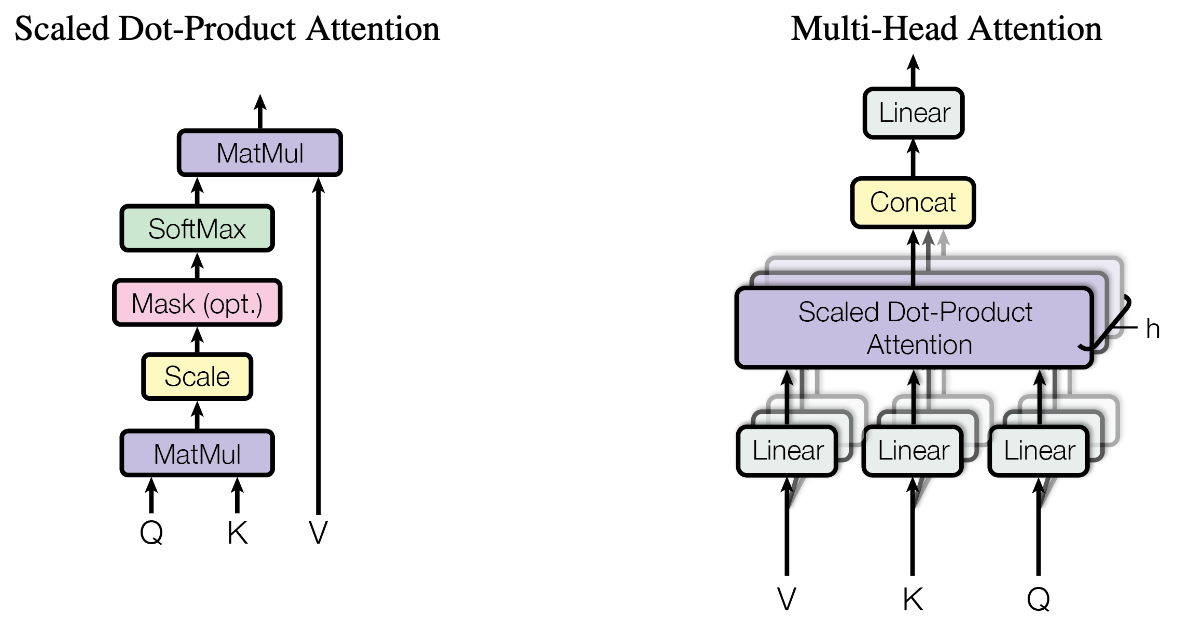
\includegraphics[width=0.8\textwidth]{figures/attentionArches.png}
    \caption[Parallel attention mechanism]{Parallel attention mechanism.\footnotemark}\label{fig:paraAttention}
\end{figure}

\footnotetext{Diagram borrowed from
    \citeauthor{attentionIsAllYouNeed},~\cite[4]{attentionIsAllYouNeed}.}

\Cref{fig:paraAttention} demonstrates how a multi head transformer based architecture
allows from greater concurrency than traditional approaches.

% \subsubsection*{Pre-training}
%
% \acrshort{llms} rely on \textit{pretraining}.
% Lorem ipsum dolor sit amet.

\subsubsection{The importance of training data}

As a conseuqence of \acrshort{llms} being statistical models of a certain input
data~\cite[1]{llmSurvey}, what data the model is trained on is of great
importance for the capabilities of the model~\cite[6]{llmSurvey}.
\citeauthor{llmSurvey} give an overview of various \acrshort{llms} and what
kinds of corpora\footnote{A corpus (pl. corpora) refers to a document
    collection.} they have been trained on~\cite[11-14]{llmSurvey}.

The training data will provide the model with its base understanding of the
world, and as such it will dictate \begin{inparaenum}
    \item what it `knows', and
    \item how we should interact with it.
\end{inparaenum}
E.g., if we want to solve problems related to software code, we should employ a
model that has been \textit{trained} on software code related topics so that the
probability of it predicting correct tokens will be higher. If it has not seen
any code during its training it would not have any base `knowledge' for solving
our problem, and its output would be bad. The \acrshort{llm} would however have
no way of knowing if its output would be right or wrong, and we could say that
it would have \textit{hallucinated}.
See \cref{sec:llmProblems} for furhter information
about hallucination.


\subsubsection{Emergent abilities}\label{sec:emergentAbilities}

\citeauthor{emergentabilitiesLLM} outline how \textit{emergent abilities} appear
when scaling up language models~\cite[1]{emergentabilitiesLLM}. They define
\textit{emergent ability} to refer to abilities that are not present in smaller
models, but present in the larger ones\cite[1]{emergentabilitiesLLM}, building
on physisist~\citeauthor{anderson1972more} stating that \textit{Emergence is
    when quantitative changes in a system result in qualitative changes in
    behavior.}~\cite[2]{emergentabilitiesLLM}.

Furhtermore, they discuss how \textit{few-shot prompting} typically can achieve
far superior results for harvesting \acrshort{llm} emergent abilities, wheras
one-shot prompting can perform worse than randomized
results~\cite[3-4]{emergentabilitiesLLM}.

They continue outlining several approaches for achieving augmented prompting
strategies, underlining how \begin{inparaenum}
    \item multi-step reasoning
    \item instruction following
    \item program execution,
    and
    \item model calibration
\end{inparaenum}
all serve as possible ways of increasing \acrshort{llm} performance~\cite[5]{emergentabilitiesLLM}.

% \tanke{Burde bygge på forrige seksjon om "små" language models}

\subsubsection{Intelligence in \acrshort{llms}}\label{sec:llmIntelligence}

There are three theories on machine intelligence, each serving to
explain how they `\textit{think}': \begin{inparaenum}
    \item stochasitc parrot
    \item Sapir-Whorf hypothesis,
    and
    \item conceptual blending.
\end{inparaenum}

\subsubsection*{Stochastic parrot}\label{sec:llmParrot}

\citeauthor{parrot} outline how \acrshort{llms} can \textit{fool} humans as they
are trained on ever larger amounts of parameters and data, appearing to be in possession of an
intelligence~\cite[610-611]{parrot}.

This anticipates the phenomenon of hallucination (\cref{sec:llmHallucination}).

\subsubsection*{Sapir-Whorf hypothesis}

The Sapir-Whorf hypothesis posits that  \textit{The structure of anyone’s native
    language strongly influences or fully determines the world-view he will acquire
    as he learns the language.}~\cite[128]{sapirWhorf}.

We note how this maps to our \acrshort{llms}, indicating that they will only ever
be able to `know' the data on which they have come into contact with.

Or: \textbf{Language} defines the possible room for \textbf{thought}.


\subsubsection*{Conceptual blending}
%Relevant?

Conceptual blending is a theory on intelligence. It refers to the basic mental
operaion that leads to new meaning or insight that occurses when one identifies
a match between to input mental spaces, to project selectively from those inputs
into a new `blended' mental space~\cite[57-58]{conceptBlending}.

This phenomenon explains how we are able to imagine phenomenonae that logically
should not exist such as \textit{land yacht} (\cref{fig:landYacht})

\begin{figure}[h]
    \centering
    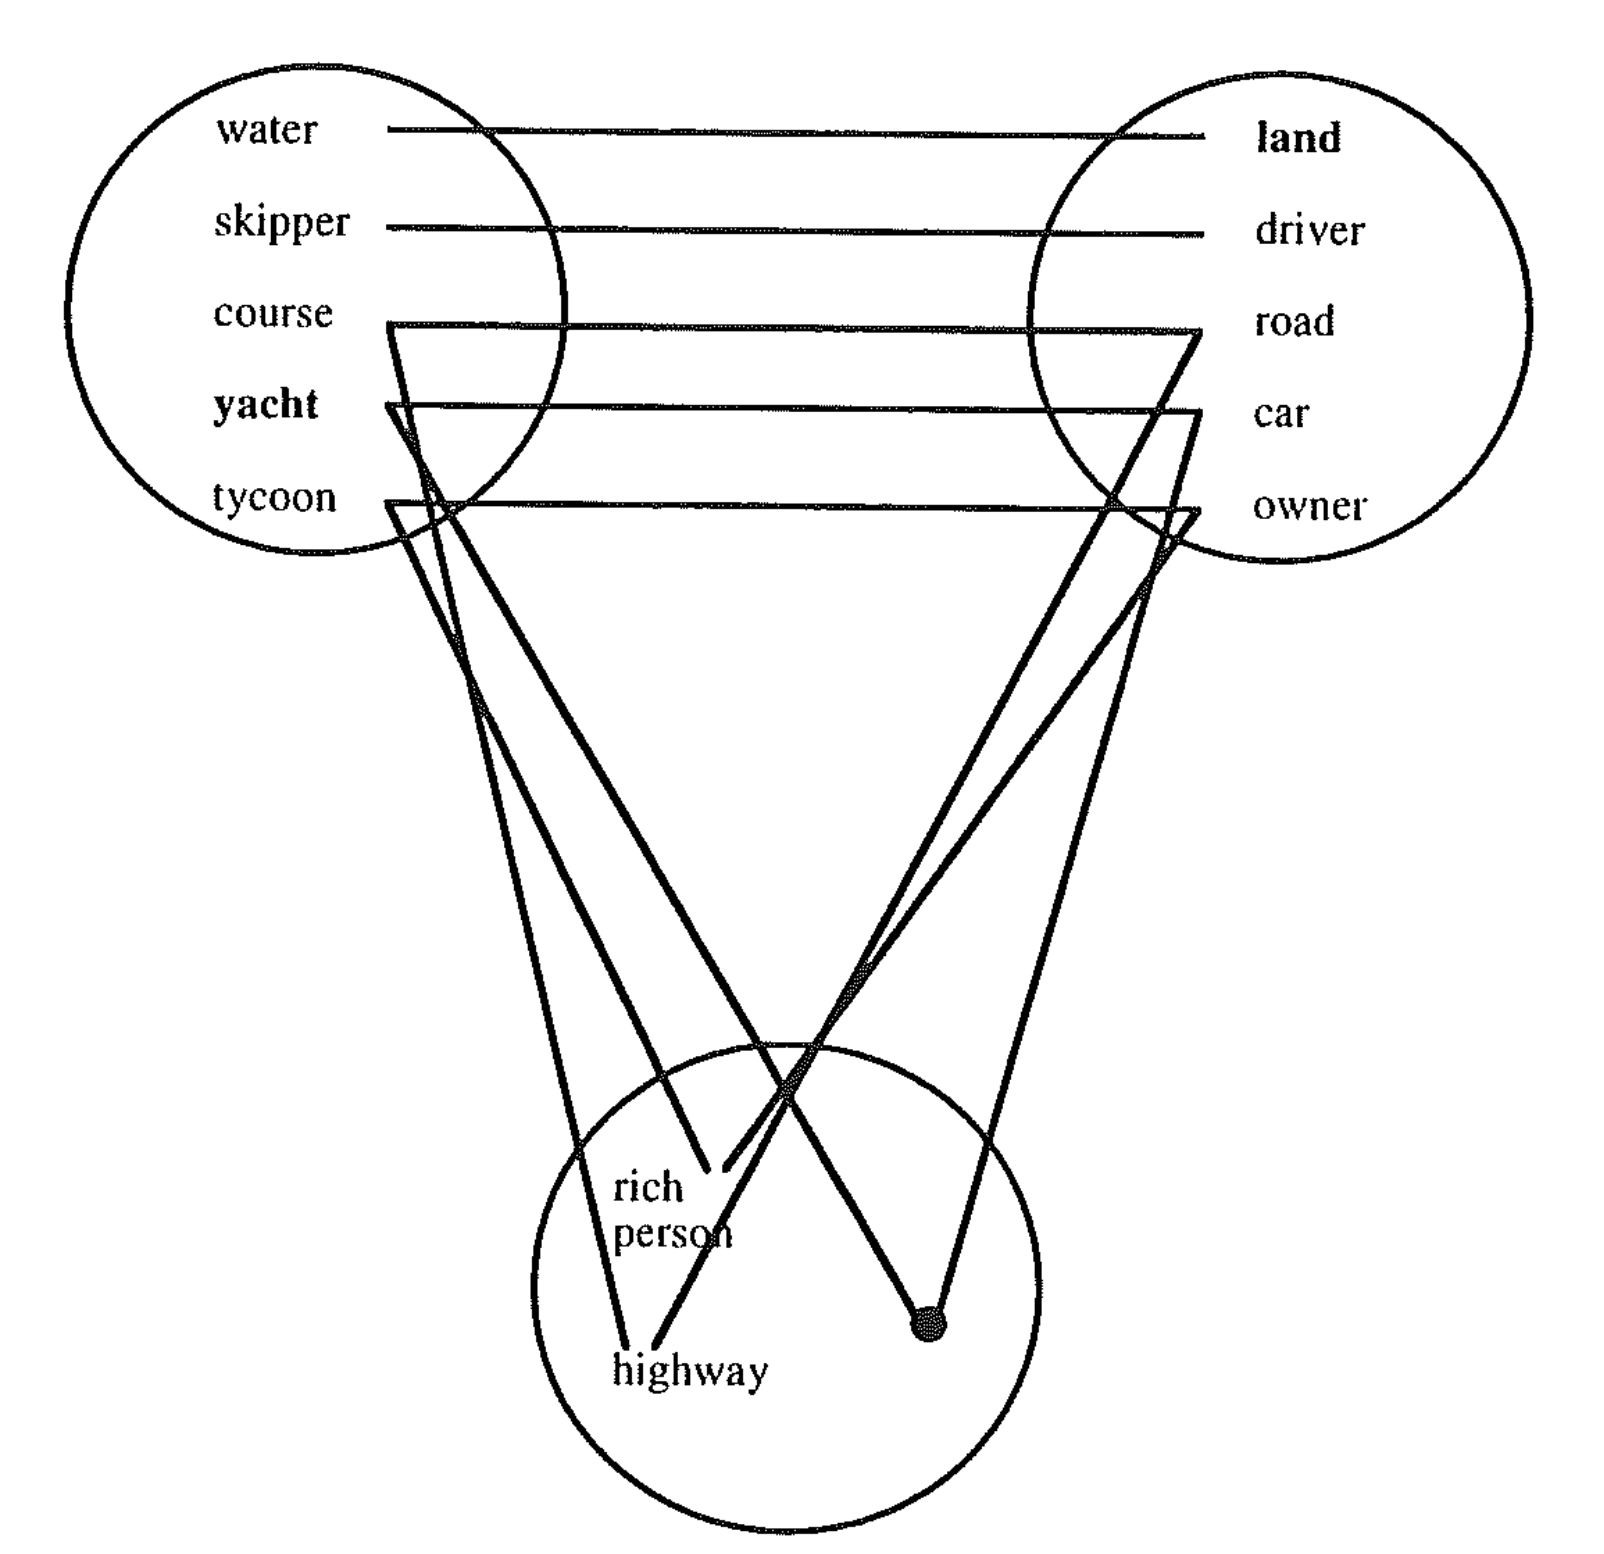
\includegraphics[width=0.8\textwidth]{figures/landYacht.png}
    \caption[Land yacht conceptual blend]{The conceptual blend of a \textit{land
            yacht}\footnotemark}\label{fig:landYacht}
\end{figure}

\footnotetext{Diagram borrowed from \citeauthor{conceptBlending},~\cite[67]{conceptBlending}.}

We note how this is how \acrshort{llms} operate when processing vectorized
linguistic data.
% Conceptual blending is a theory on both machine and human intelligence. 


\subsubsection{Utilising \acrshort{llms} - Prompt engineering}\label{sec:llmUtilization}


A typical way of interacting with \acrshort{llms} is \textit{prompting}~\cite[44]{llmSurvey}. You
prompt the model to solve various tasks. As we saw in \cref{sec:emergentAbilities}, the level of
performance you are able to extract from your \acrlong{llm} can depend a great deal on how you
interact with it. The process of manually creating a suitable prompt is called \textbf{prompt
    engineering}~\cite[44]{llmSurvey}.~\citeauthor{llmSurvey} outline three principal prompting
approaches:

\textbf{\acrfull{icl}} is a representative prompting method that formulates the task
description and/or deminstrastions in natural language text~\cite[44]{llmSurvey}. It is based on
\textit{tuning-free prompting} and it, as the name implies, never tunes the parameters of the
\acrshort{llm}~\cite[15]{promptingSurvey}. One the one hand, this allows for efficiency, but on the
other hand, heavy engineering is typically required to achieve high accuracy, meaning you must
provide the \acrshort{llm} with several answered prompts~\cite[16]{promptingSurvey}. In layman's
terms, \acrshort{icl} entails including examples of the process you want the model to perform when
prompting it.

\textbf{\acrfull{cot} prompting} is proposed to enhance \acrlong{icl} by involving a
series of intermediate reasoning steps in prompts~\cite[44, 52]{llmSurvey}. The basic concept of
\acrshort{cot} prompting, is including an actual \acrlong{cot} inside the prompt that shows the way
form the input to the output~\cite[52]{llmSurvey}.~\citeauthor{llmSurvey} note that the same effect
can be achieved by including simple instructions like `\textit{Let's think step by step}' and other
similar `magic prompts' in the prompt to the \acrshort{llm}, making \acrshort{cot} prompting easy to
use~\cite[52]{llmSurvey}.

\textbf{Planning} is proposed for solving complex tasks, which first breaks them down into smaller
sub-tasks and then generates a plan of action to solve the sub-tasks one by
one~\cite[44, 54]{llmSurvey}. The plans are being generated by the \acrshort{llm} itself upon
prompting it, and there is a distinction between text-based and code-based approches. Text-based
approches utilise natural language, wheras code-based approches utilise executable computer code~\cite[54-55]{llmSurvey}.


\subsubsection{General challenges with \acrshort{llms}}\label{sec:llmProblems}

We have seen that \acrshort{llms} demonstrate promising abilities
(\cref{sec:emergentAbilities} \& \cref{sec:llmIntelligence}) But they have nevertheless
certain issues attached to them that we need to be aware of.

\subsubsection*{Hallucination}\label{sec:llmHallucination}

As we saw in \cref{sec:llmParrot}, \acrshort{llms} are prone to
\textit{bullshitting}. They have no intuition of, or concern with \textit{the
    truth}. They only ever yield whatever response is the most probable under their
\textsc{beam search} algorithm being applied on their training data.

\subsubsection*{Environmental concerns}

\acrshort{llms} are awful for the environment. They consume wast amounts of \begin{inparaenum}
    \item power,
    and
    \item water,
\end{inparaenum}
eating up the resources for human communities.

\citeauthor{llmCarbon} did however find that spefically Co2-emissions can be
significantly lower for \acrshort{llms} than humans for specific
tasks~\cite{llmCarbon}. They did however fail to consider other relevant factors such
as water consumption.


\subsubsection{The different kinds of \acrshort{llms}}\label{sec:llmJungle}

There are several available \acrshort{llms}, some of which are open source, and some proprietary.
Open source \acrshort{llms} afford greater insight into their composition and underlying training
data, wheras proprietary models appear more like black boxes. Some popular model families include
the GPTs, Gemeni, Llama, Claude, Mistral, and DeepSeek.

The \acrshort{llms} differ primarily in their \begin{inparaenum}
    \item parameters, and
    \item training data.
\end{inparaenum}
As we saw in \cref{sec:llmArch}, all typical \acrshort{llms} utilise a transformer-based neural
network. But due to their various different properties, different models can behave differently for
different tasks regardless of their similar architecture.

What they all share is their ability to perform \textit{inference}, meaning that they predict output
tokens given some input tokens (see \cref{sec:llmParrot,sec:llmHallucination}).

\subsection{Existing \acrshort{llm} applications for \acrshort{ads}}\label{sec:llmsForAds}


\citeauthor{LLM4AD} give a broad overview of some of the ways \acrshort{llms} have been applied for
\acrshort{ads}, highlighting some of the opportunities and potential weaknesses of \acrshort{llm}
applications for \acrshort{ad} purposes. One of the ways \acrshort{llms} can be applied, is for
adjusting the driving mode, or aiding in the decision-making
process~\cite[1]{LLM4AD}.~\citeauthor{driveAsYouSpeak} delve further into these aspects in their
other work \citetitle{driveAsYouSpeak}, providing a framework for integrating \acrlong{llm}'s
\begin{inparaenum}
    \item natural langauge capabilities,
    \item contextual understanding,
    \item specialized tool usage,
    \item synergizing reasoning, and
    \item acting with various modules of the \acrshort{ads}
\end{inparaenum}~\cite[1]{driveAsYouSpeak}.